\section{Background and Problem Setting} \label{sec:background}

We start with background on latent variable graphical models and discuss the theoretical model we analyze. We explain the two stages of how to produce labels with it---learning the label model and aggregating sources---for both the labeled and weakly-labeled data cases, and then conclude with label model evaluation and the key challenges.


\begin{figure*}
    \centering
    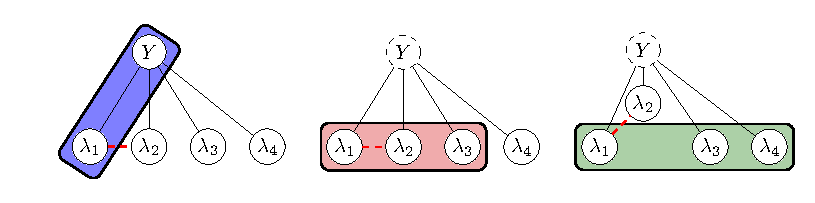
\includegraphics[width=.7\textwidth]{figures/models.pdf}
    %
    \caption{Latent variable models with unmodeled dependency (red edge), leading to misspecification. Boxes indicate observable variables used for accuracy estimation. Left: model with access to label $Y$. Pairs $(\lambda_i, Y)$ directly estimate source accuracy. Center: latent model with unobserved $Y$. Triplet (red) includes unmodeled dependency, leading to inconsistent estimation. Right: Corrected model using medians. Triplet excludes the dependency, returning to consistency.}
    \label{fig:biases}
\end{figure*}

%In this section, we provide background on the weak supervision problem setting, the graphical model assumptions for the true distribution as well as the misspecified model used, and the method-of-moments approach commonly used to learn model parameters when labeled data is unavailable.  

%This work explores when and how a small number of labeled data points can be used to improve the quality of noisy labels produced by the data programming pipeline. In Section \ref{sec:setting_dp} we provide background about data programming and methods for combining labeling functions. In Section \ref{sec:setting_adding_labels} we describe the modified setting where some labeled data is available. Finally, we discuss evaluating data programming methods in Section \ref{sec:setting_evaluation}.

%\subsection{Background: Data Programming}
%\label{sec:setting_dp}

\paragraph{Setup} In weak supervision frameworks, e.g., data programming \citep{Ratner16}, a labeled dataset is built by acquiring noisy sources operating on unlabeled data. %The outputs of these sources %. Often a programmatic heuristic written by practitioners, each weak source either votes or abstains on a data point, thus overall producing multiple noisy labels per point that are then
%are aggregated by a \emph{label model} to output the training label for each point. 
The usual input is a supply of $n_U$ unlabeled data points; in our setting, we also consider a smaller \emph{labeled} dataset of $n_L$ samples as well. The output is a large, labeled dataset.

Let $X \in \X$ and $Y \in \mathcal{Y} = \{-1, 1\}$ with $(X, Y)$ from some distribution $\D$. We consider an unlabeled dataset $\bm{X}_U = \{x_i^U\}_{i = 1}^{n_U}$ and a labeled dataset $(\bm{X}_L, \bm{Y}_L) = \{(x_i^L, y_i^L) \}_{i = 1}^{n_L}$ drawn from $\D$.
There are $m$ weak sources, each
voting on $X$ via a deterministic \textit{labeling function} (LF)
$\lf_j: \X \rightarrow \mathcal{Y} \cup \{0\}$ for all
$j = 1, \dots, m$ ($\lf_j(X) = 0$ is an abstain). 
For each $X$, our goal is to use the outputs of $\bm{\lf}$, the vector of LFs, to construct a model to infer $Y$.

To aggregate the noisy outputs of $\bm{\lf}$, we learn the joint distribution $\Pr(Y, \bm{\lf})$, called the \textit{label model}. It combines votes into soft labels $\widetilde{y}_i := 2 \Pr(Y = 1 | \bm{\lf} = \bm{\lf}(x_i)) - 1 \in [-1, 1]$ for each $x_i$ by applying
the $m$ sources to $\bm{X}_U$ and $(\bm{X}_L, \bm{Y}_L)$. These labels can then be used for prediction, or as training data for a downstream model. The overall approach is thus a two-step process: (i) learn the label model probabilities (using labeled or unlabeled data), and (ii) compute $\tilde{y}_i$ for unlabeled points.

%We use the label model outputs as the final predictions for $Y$ such that its generalization error precisely captures the effect of model misspecification and labeled versus unlabeled data. However, the labels are often used to train an additional end model, for which our analysis on the quality of training data is still valid.

% \paragraph{Misspecification in weak supervision}
% To learn the joint distribution $\Pr(Y,\bm{\lf})$, we typically assume that there exist subsets of labeling functions that are conditionally independent given $Y$. When 

\paragraph{Theoretical model}
We pick a simple theoretical model that captures many WS settings and still presents all of the challenges for comparing between the types of data. We assume an Ising model for $\Pr(Y, \bm{\lf})$; the only difference between the labeled and weakly labeled setting is that $Y$ is latent in the latter. %Following the standard notation,
%We present the standard graphical model assumptions for the true distribution $\Pr(Y, \bm{\lf})$. Then, we discuss the misspecified graphical model used in weak supervision and how it outputs labels.
The set of canonical parameters is $\Theta$, and the dependency graph is $G = (V, E)$, where $V = Y \cup \bm{\lf}$ and $E$ consists of edges from $Y$ to the labeling functions as well as the $d$ edges among the labeling functions, $E_{\lf}$. %The graph $G$ specifies dependencies using standard technical notions from the PGM literature~\citep{koller2009probabilistic, Lauritzen, wainwright2008graphical}. 
Recall that the lack of an edge in $G$ between a pair of
variables indicates independence conditioned on a separator set of
variables~\citep{Lauritzen}, so the true distribution can be modeled as
\begin{align}
    \Pr(Y, \bm{\lf}) = \frac{1}{Z} \exp \Big(\theta_Y + \sum_{i = 1}^m \theta_i \lf_i Y + \sum_{(i, j) \in E_{\lf}} \theta_{ij} \lf_i \lf_j \Big),
    \label{eq:true_pgm} \nonumber 
\end{align}
with cumulant function $Z$. For cleaner presentation, we assume that $\Theta \ge 0$ (i.e. no LFs that disagree with other LFs or $Y$ on average) and $E_{\lf}$ is sparse enough such that $\text{deg}(\lf_i) \le 2$ for all $\lf_i$, e.g. each LF is conditionally dependent on at most one other LF. This can lead to model misspecification when edges are unknown.

%With this, we can explain the two steps involved in the process.

\paragraph{Aggregation} The probabilistic label on $X$ is computed using a Naive Bayes approach that assumes all labeling functions are conditionally independent with $E_{\lf} = \emptyset$:
\begin{align}
    \widetilde{\Pr}(Y &= 1 | \lf = \lf(X)) \\
    &= \frac{\prod_{i = 1}^m \widetilde{\Pr}(\lf_i = \lf_i(X) | Y = 1) \Pr(Y = 1)}{\hat{\Pr}(\lf = \lf(X))} 
    \label{eq:inference}
\end{align}
where the class balance $\Pr(Y = 1)$ is assumed to be known, $\hat{\Pr}$ is an empirical probability
%\bcw{This still makes me a little uncomfortable. You'd never use the empirical counts of $\lambda$ in practice, because the number of times a particular set of labeling function outputs appears decays exponentially with $m$, which means our estimates will be pretty terrible. Not sure what can be done about this though, given that the error decomposition seems like it leans on this expression for the probabilistic label pretty heavily.}
, and $\widetilde{\Pr}$ indicates an estimated probability resulting from the label model estimation step described below. %The class balance $\Pr(Y = 1)$ is assumed to be known, so the only term to be estimated is $\widetilde{\Pr}(\lf_i = \lf_i(X) | Y = 1)$ for each $\lf_i$, which we describe how to do below. 
%
In practice, the conditional independence assumptions required for (\ref{eq:inference}) may not hold, but dependencies among labeling functions are often unknown%\footnote{We discuss techniques to rectify this and their costs at the end of the following section.}
. Therefore, conditional independence is assumed---and so we may suffer from \emph{misspecification} in inferring our probabilistic labels. %In the following we compute the cost of this error and its implications for the value of data. 

%Note that in the case of labeled data, we can compute this directly, but for unlabeled data, we estimate this probability using the graphical model structure.

\paragraph{Learning the label model: labeled vs. weakly labeled data}
For the labeled dataset, we can estimate $\widetilde{\Pr}(\lf_i = \lf_i(X) | Y = 1)$ in (\ref{eq:inference}) directly from samples, as $Y$ is observed. 

In the weakly-labeled case, %a different approach is taken. W
we consider method-of-moments estimators that exploit the independence properties of the Ising model. While there are several choices for this step, we use the approach described in \cite{fu2020fast}, which relies on the property of our Ising model
%\begin{proposition}
that if $\lf_i \independent \lf_j | Y$, then $\lf_i Y \independent \lf_j Y$.
%\label{prop:triplet}
%\end{proposition}
%
This implies that $\E{}{\lf_i Y} \cdot \E{}{\lf_j Y} = \E{}{\lf_i \lf_j Y^2} = \E{}{\lf_i \lf_j},$ which is directly estimable.
Define $a_i := \E{}{\lf_i Y}$ as the unknown \textit{accuracy} of $\lf_i$. If we can introduce a third $\lf_k$ that is conditionally independent of $\lf_i$ and $\lf_j$, we have a system of equations that can be solved using observable rates of agreement among LFs. We thus use this \textit{triplet method} to recover these accuracies; in particular, this is a method-of-moments approach in which we choose two $\lf_j$, $\lf_k$ at random for each $\lf_i$ and solve up to sign:
\begin{align}
    |\widetilde{a}_i^{(j, k)}| := \sqrt{\bigg| \frac{\Ehat{\lf_i \lf_j} \Ehat{\lf_i \lf_k}}{\Ehat{\lf_j \lf_k}} \bigg|},
    \label{eq:triplet}
\end{align}
where $\hat{\mathbb{E}}$ represents empirical estimates of the expectations %using the weakly labeled dataset $\bm{X}_U$. 
We then use the estimated $\widetilde{a}_i^{(j, k)}$ to directly compute $\widetilde{\Pr}(\lf_i = \pm 1 | Y = 1)$ for \eqref{eq:inference}. However, randomly choosing $\lf_j$ and $\lf_k$ may not satisfy conditional independence, and thus we incur further error in estimating accuracies due to misspecification---in a way unique to the weakly labeled setting. We aim to capture this error in our evaluation. % The following section characterizes this notion.

\paragraph{Evaluating the model}

We define the label model's generalization error as $R = \mathbb{E}_{(Y, \bm{\lf}), \N, \tau}[l(\widetilde{Y}, Y)]$ where expectation is taken over the distribution of $(Y, \bm{\lf})$, $\N$ (the random dataset used), and $\tau$ (the algorithmic randomness, i.e. the triplets in the weakly-labeled case). $l(\cdot, \cdot)$ here is the cross entropy loss 
%\steve{maybe move this up to the beginning of the paragraph, so the ordering is more natural?}
, defined on a point $(x_i, y_i)$ as
\begin{align*}
l(\widetilde{y}_i, y_i) = &-\frac{1 + y_i}{2} \log \widetilde{\Pr}(Y = 1 | \lf = \lf(x_i)) \\
&- \frac{1 - y_i}{2} \log \widetilde{\Pr}(Y = -1 | \lf = \lf(x_i)).
\end{align*}

We let $R_U$ denote the error for the weakly-labeled dataset and $R_L$ for labeled.

\paragraph{Key Technical Challenges}
The goal of our evaluation framework is to answer questions such as
\begin{itemize}
    \item The weakly labeled case computes the function (\ref{eq:triplet}) of empirically observable quantities, while the labeled case accesses them directly---how do the errors due to sampling noise compare? 
    \item Which stage of the pipeline---learning the label model and aggregation---does misspecification impact, and how does this differ between the cases?
    %\item How to price $n_L$ labeled samples in terms of the cheaper weakly labeled ``currency''?
\end{itemize}


%%%%%%%%%%%%%%%%%%%%%%%%%%%%%%%%%%%%%%%%%%%%%%%%%%%%%%%%%%%%%%%%%%%%%%%%%%%%%%%%%%%%%%%%%%



%We define the data programming task for binary classification as follows. Let $X\in\mathcal{X}$ for some set $\mathcal{X}$ of possible inputs and $Y\in\{-1,1\}$ where $(X,Y)\sim\mathcal{D}$ for some distribution $\mathcal{D}$. We are given an unlabeled dataset $\boldsymbol{X}_U=\{x^i_U\}_{i=1}^{n_U}$ with corresponding unobserved gold labels $\boldsymbol{Y}_U=\{y^i_U\}_{i=1}^{n_U}$ where $(x^i_U,y^i_U)$ are i.i.d. samples from $\mathcal{D}$. We are also given $m$ labeling functions $\lambda_1,\hdots,\lambda_m$ where $\lambda_j:\mathcal{X}\to\{-1,0,1\}$ with an output of $0$ denoting that the labeling function \textit{abstains} (does not provide an answer). We say that a labeling function \textit{fires} when it does provide an answer. Labeling functions are typically fairly accurate but only fire on a small fraction of points. Our goal is to use our $m$ labeling functions to produce noisy labels $\tilde{\boldsymbol{Y}}=\{\tilde{y}^i\}_{i=1}^{n_U}$ with $\tilde{y}^i\in[-1,1]$ representing our confidence about the gold label (for example, the probabilistic label might be closer to $0$ if labeling functions disagree). These noisy labels can then be used as training data.


%Aggregating labeling function outputs usually involves estimating the \textit{accuracy} and \textit{coverage} of each labeling function from \textit{only unlabeled data} and then weighting labeling functions according to these two parameters. The accuracy $\alpha_j$ of the $j$'th labeling function is the accuracy over the points where it fires and the coverage $\beta_j$ of the $j$'th labeling function is the fraction of points where it fires.
%\begin{equation}
%\alpha_j=\text{Pr}[\lambda_j(X)=Y\mid\lvert\lambda_j(X)\rvert=1]
%   \quad\text{and}\quad 
%\beta_j=\text{Pr}[\lvert\lambda_j(X)\rvert=1]
%\end{equation}
%Several methods have been proposed for estimating accuracies and coverages, including marginal maximum likelihood estimation, completing the covariance matrix between labeling function outputs and the unobserved true labels, and solving for the accuracies of three labeling functions (for which a closed-form solution exists) at a time \citep{alex2016data, ratner2019training, fu2020fast}. While estimating coverages from unlabeled data is easy, estimating labeling function accuracies requires making assumptions about their behavior. Most previous methods assume that labeling functions are conditionally independent given the gold label, that is
%\begin{equation}
%    \text{Pr}[\lambda(X)=\boldsymbol{z}\mid Y=y]=\prod_{j=1}^m\text{Pr}[\lambda_j(X)=z_j\mid Y=y]
%\end{equation}
%Efforts have been made to learn dependencies between labeling functions \citep{bach2017learning, varma2019learning} and previous data programming methods propose model variants which permit dependencies, but they ultimately rely on subsets of conditionally independent labeling functions to estimate accuracies. Furthermore, models which assume that all labeling functions are conditionally independent, such as the base model from \cite{Ratner_2017}, are in practice often used out-of-the-box. Therefore, in this work we study data programming models which assume that all labeling functions are conditionally independent.

%\subsection{Adding labeled data to the data programming setup}
%\label{sec:setting_adding_labels}

%For this work, we modify the standard data programming setup such that in addition to labeling functions the expert provides a small number of labeled data points. Our task is the same as above, except that we are also given a labeled dataset $\boldsymbol{X}_L=\{x^i_L\}_{i=1}^{n_L}$ with observed gold labels $\boldsymbol{Y}_L=\{y^i_L\}_{i=1}^{n_L}$ where again $(x^i_L,y^i_L)$ are i.i.d. samples from $\mathcal{D}$. We are interested in settings where the labeled dataset size $n_L$ is much smaller than the unlabeled dataset size $n_U$ because if $n_L$ is close to $n_U$ supervised or semi-supervised approaches would likely perform well and data programming would not be necessary.

%\subsection{Evaluating noisy labels directly}
%\label{sec:setting_evaluation}

%Generally in data programming the quality of the noisy training labels is measured by training an \textit{end model} on these labels and evaluating its performance on a test set. Because the end model performance is dependent on the choice of architecture and generally correlates with the quality of the noisy labels, we instead directly measure the accuracy of the noisy labels. In our modified setting, the labels $\boldsymbol{Y}_L$ are given for the subset $\boldsymbol{X}_L$ of the training data so we evaluate noisy labels produced for an unseen test set. We define accuracy of noisy labels $\tilde{\boldsymbol{Y}}_\text{test}=\{\tilde{y}_\text{test}^i\}_{i=1}^{n_\text{test}}$ where $\tilde{y}_\text{test}^i\in[-1,1]$ with true test labels $\boldsymbol{Y}_\text{test}=\{y_\text{test}^i\}_{i=1}^{n_\text{test}}$ where $y_\text{test}^i=\{-1,1\}$ as follows (with predictions of $0$ considered ``half'' correct).
%\begin{equation}
%    A(\boldsymbol{Y}_\text{test},\tilde{\boldsymbol{Y}}_\text{test})=\frac{1}{n_\text{test}}\sum_{i=1}^{n_\text{test}}\begin{cases}
%        1&\text{ if }\text{sign}(\tilde{y}_\text{test}^i)=y_\text{test}^i\\
%        1/2&\text{ if }\tilde{y}_\text{test}^i=0\\
%        0&\text{ otherwise}
%    \end{cases}
%\end{equation}

